Už jsme viděli, jak použít Darbouxovu vlastnost a \uv{půlení intervalů} na optimalizaci.
Ale to nemusí být vždy praktické:
\begin{itemize}

	\item  Rychlost konvergence\ldots

	\item  Jak ten postup zobecníte na funkce více proměnných?

\end{itemize}

Zkusme se podívat na následující funkci a najít její minimum fyzikální úvahou:
$$f(x) = x^4 - 3x^3 + 2$$

Analytickými metodami umíme snadno najít minimum (vyšetříme první a druhé derivace, vzpomeneme si na věty z přednášky a jsme hotovi).
(Obrázek~\ref{fig:gradient_descend}).
\begin{figure}[H]
	\centering
	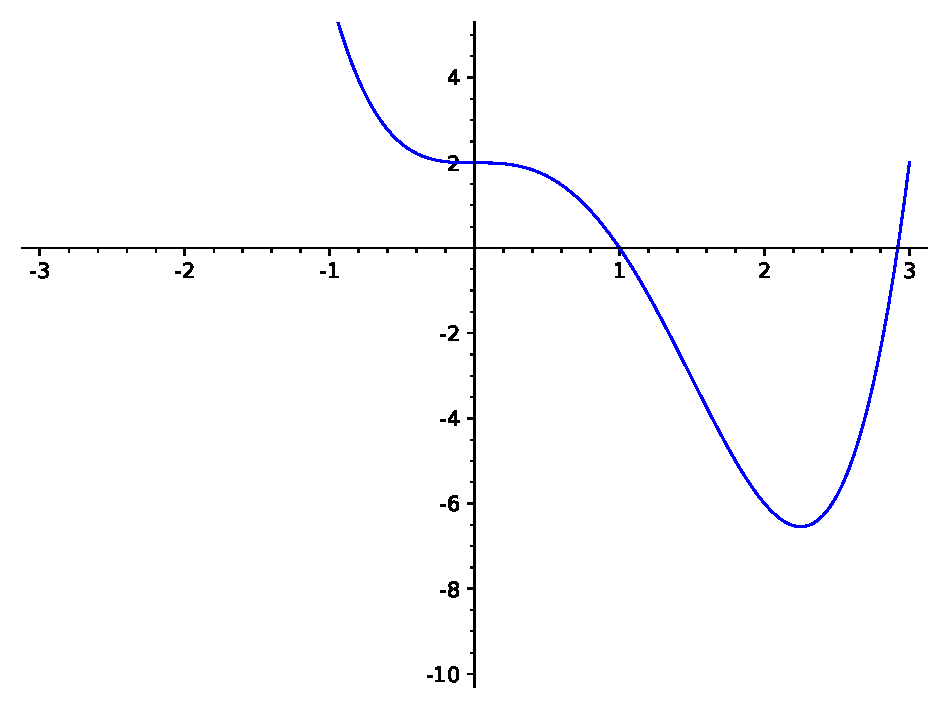
\includegraphics{bonus/fig/gd.pdf}
	\caption{$f(x) = x^4 - 3x^3 + 2$}
	\label{fig:gradient_descend}
\end{figure}

\textbf{Myšlenka:} co by se stalo, kdybychom po grafu pustili kuličku?

\textbf{Pozorování:} skutálí se dolů do minima!

\textbf{Otázka:} ale kudy je dolů?

Derivaci téhle funkce umíme vyhodnotit snadno: $f'(x) = 4x^3 - 9x^2$.
\begin{itemize}
	\item  Pokud je derivace záporná, funkce klesá.
	\item  Pokud je derivace kladná, funkce roste.
\end{itemize}

Dokonce platí něco lepšího:
\begin{itemize}
	\item  Pokud je derivace \emph{hodně} záporná, funkce \emph{hodně} klesá.
	\item  Pokud je derivace \emph{hodně} kladná, funkce \emph{hodně} roste.
\end{itemize}

Takže když chceme minimalizovat, děláme tohle:
\begin{itemize}
	\item  Pokud je derivace (hodně) kladná, jdeme (hodně) vlevo.
	\item  Pokud je derivace (hodně) záporná, jdeme (hodně) vpravo.
\end{itemize}

To zní dobře, protože v extrému je derivace nulová (nebo neexistuje, ale to teď zanedbáme), takže se nepohneme nikam.

Jednodušeji řečeno: odečteme derivaci.

Jednoduchý Python kód:
\inputminted{python}{bonus/gd.py}
Výstup:
\texttt{\\
current = 4.0\\
current = 2.88\\
current = 2.67098112\\
current = 2.55084758768784\\
current = 2.4725451025639247\\
current = 2.4181241075908217\\
current = 2.3788010610759907\\
current = 2.349647226900712\\
current = 2.3276417627201864\\
current = 2.3108155002345616\\
current = 2.297825629818595\\
current = 2.2877248517791187\\
current = 2.279827252147626\\
current = 2.2736260324425532\\
current = 2.2687407592672773\\
current = 2.2648822733430056\\
current = 2.2618286143740107\\
current = 2.2594080688614797\\
current = 2.2574869694912945\\
current = 2.2559607515339213\\
Minimum at: 2.254747295376156
}

Připomeňme, že skutečné minimum je 2.25.

\emph{
	Zkuste si pohrát s tím kódem.
}
Problémy, které mohou nastat:
\begin{itemize}

	\item  Zasekneme se v inflexním bodě. Tohle se snad nestane (\uv{vratká pozice}).

	\item  Příliš velké alpha můžeme ulítnout (poskakujeme zleva doprava čím dál tím větší skoky).
		Tohle bývá problém, proto se občas postupně snižuje alpha, ke kroku se přičte i nějaký malý násobek předchozího kroku\ldots
		Spousta heuristik, které běží lépe.
		Nad rámec tohoto povídání.

	\item  Málo iterací -- no tak poběžíme více iterací (tzn. déle).

\end{itemize}

